\section{Introduction}
\label{sec:introduction}
\begin{figure*}[t]
\centering
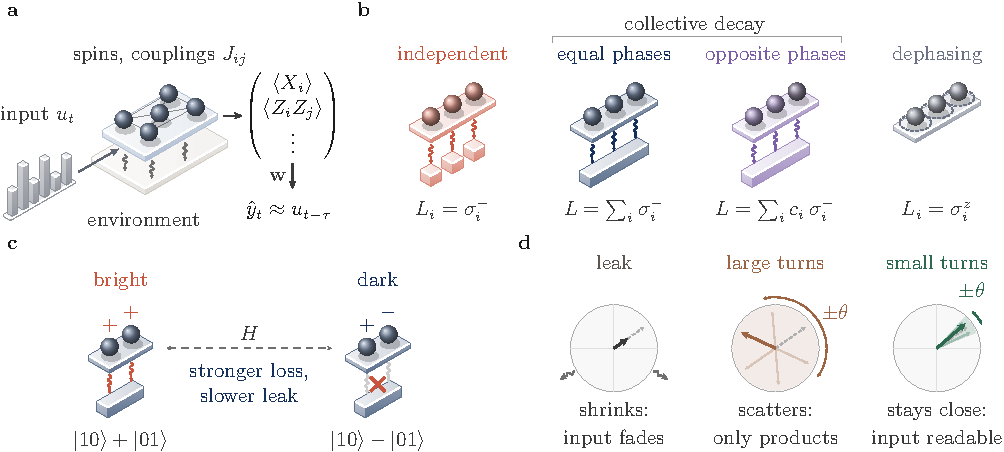
\includegraphics[width=\textwidth]{figures/fig1_concept.pdf}
\caption{\textbf{Engineering how a quantum reservoir leaks.}
\textbf{a}~Inputs drive interacting spins, and a trained linear readout recalls past inputs.
\textbf{b}~Four forms of dissipation with the same total coupling. The darker spins couple with the opposite sign.
\textbf{c}~Two spins on one channel: their decays add (bright) or cancel (dark), and strong loss holds them in the
dark state, the quantum Zeno effect.
\textbf{d}~A stored signal fades because it leaks away or because later inputs turn it at random.}
\label{fig:concept}
\end{figure*}

Processing information over time requires a memory of what came before. A physical system can provide such a memory
because each input changes its state and leaves traces that influence its later response. Reservoir computing uses these
traces to perform a task: an input stream drives a dynamical system, and a weighted sum of quantities describing its
state produces the output. Only these weights are trained; this mapping is called a linear
readout~\cite{Maass2002,JaegerESP2001}. In quantum reservoir computing (QRC), the evolving system is quantum mechanical,
and the readout uses quantities obtained by measuring it~\cite{Fujii2017}. The challenge is to keep earlier inputs
accessible while new information continues to arrive.

The environment shapes how these traces fade. A system can lose energy or information to its surroundings through
processes collectively described as
dissipation~\cite{ChenNurdin2019,Chen2020,Sannia2024,Ricci2026,Domingo2023,Goetting2025,Mujal2023,Franceschetto2026,KobayashiFeedback2024,Cindrak2024,Sannia2026Memory,Paparelle2026}.
Previous work has shown that tuning the dissipation rate improves memory, in some reservoirs with the best performance
at an intermediate loss rate~\cite{Sannia2024,Goetting2025}. Input, interactions, and dissipation can also be optimized
together~\cite{MartinezPenaPRL2021,Baumann2026}. The rate specifies how strongly the environment acts, but the way it
acts is a separate design choice. Engineering this interaction can prepare and protect selected quantum
states~\cite{Poyatos1996,Verstraete2009,Pastawski2011,Harrington2022}. For a system processing an ongoing input stream,
this raises the possibility of controlling which traces of the past survive.

This distinction becomes concrete for a reservoir of interacting spins, each a two-level quantum system. When the spins
decay through separate routes into the environment, they undergo independent decay. When they share a common route, they
undergo collective decay. In certain joint states, the different emission paths interfere and cancel, preventing decay
through that shared route. These protected states are called dark
states~\cite{Dicke1954,AsenjoGarcia2017,Facchinetti2016}. Internal dynamics can still move the system into states that
do decay. If this decay is sufficiently rapid, however, it suppresses those transitions, a phenomenon known as the
dissipative quantum Zeno effect~\cite{FacchiPascazio2002,Zanardi2014,Burgarth2019,Reiter2012}. Stronger loss
therefore slows the escape of information from the protected states (Fig.~\ref{fig:concept}c).

A long-lived state is not yet a usable memory, because each new input changes the same state that stores the past.
A signal that initially depends on one input comes to depend on combinations of several inputs, such as their
product. This mixing is useful for tasks that require relationships between inputs, but it reduces the capacity
available for recalling single inputs~\cite{Dambre2012,Inubushi2017,Cindrak2026}. Reading the memory has a cost as
well, because resolving a weak quantum signal requires repeated preparation and
measurement~\cite{Mujal2023,Cindrak2024,Hu2023}, and a long-lived memory is hard to read if its signal is faint.
Previous work has established memory limits in classical reservoirs~\cite{JaegerESP2001,White2004,Ganguli2008},
explored input strength~\cite{Jaeger2007Leaky}, and investigated how noise and protected states affect quantum
information processing~\cite{Kubota2023,Fry2023,Cheamsawat2025,Akshay2026}. Closest to our work,
Ref.~\cite{Sannia2024} tunes the dissipation rate of the reservoir we study, Ref.~\cite{Cindrak2026} finds one
trade-off between memory and nonlinearity across reservoir schemes, and Ref.~\cite{Akshay2026} reads the output of a
reservoir from a decoherence-free subspace to classify quantum states. The Zeno protection of dark states and the
benefit of a weak input for linear memory are established. How protection, continued input, and measurement together
determine the part of the past that a readout recovers is open.

% Fig. 2 is declared here so that it lands on the top of the third page
\begin{figure*}[!t]
\centering
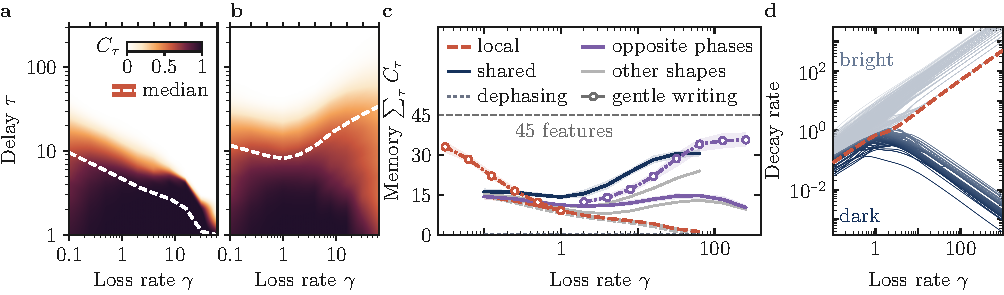
\includegraphics[width=\textwidth]{figures/fig2_clock.pdf}
\caption{\textbf{The decay structure decides whether loss shortens or prolongs the memory.}
\textbf{a,b}~Recall of the input $\tau$ steps back: stronger loss pushes it to shorter delays with independent decay
(a) and to longer delays with the equal-phase channel (b).
\textbf{c}~Linear memory capacity of all channels. Shading marks loss stronger than the couplings
($\gamma>1$).
\textbf{d}~With the equal-phase channel the dark modes decay more slowly as the loss grows, while the slowest mode
of independent decay (dashed) decays faster.}
\label{fig:clock}
\end{figure*}

Here we show that the form of the dissipation sets three properties of a memory (Fig.~\ref{fig:concept}): how long a
stored signal survives, whether and how strongly an input can be written into it, and how strong a signal is left to
measure. First, the decay channel decides at equal total coupling whether stronger loss shortens or prolongs the
memory lifetime. Independent decay shortens it, and collective decay prolongs it through dark states
(Sec.~\ref{sec:clock}). Second, mixing limits how strongly an input can be written. We prove that at a fixed input
amplitude a stored
signal combines on average $s\,t_{\mathrm{mem}}$ inputs, where the mixing fraction $s$ is the part of the stored
signal that one input disturbs and $t_{\mathrm{mem}}$ is the memory lifetime (Sec.~\ref{sec:mixing}). We also prove
that an amplitude that falls as $1/\sqrt{t_{\mathrm{mem}}}$ removes this limit. The share of single inputs then
converges to a value that depends on the input only through its squared amplitude times the lifetime, and this limit
agrees with the five-spin results without a fitted parameter. The phases with which the spins couple to a collective
channel decide whether an input reaches the dark states at all (Sec.~\ref{sec:writing}). Third, the state that the
dissipation leaves behind sets the size of the signal that measurements must resolve. At strong loss a
collective channel whose phases differ from those of the input field recovers the most memory at every measurement
budget, and where the loss can be made weak, independent decay recovers more still (Sec.~\ref{sec:price}).

Together, these results connect the physical survival of information to what a readout recovers from it. The
protection relies on quantum interference, whereas the two theorems hold for every reservoir that meets their
conditions, classical ones included, and give the size of the trade-off between memory and nonlinearity. The form of the
dissipation, the input amplitude and the measurement budget become joint design parameters, and the memory that a
readout recovers becomes a quantity that can be engineered in physical systems that process information over time.
